% main.tex
\documentclass[10pt,a4paper]{ctexbook}
\usepackage{makeidx} % 调用 makeidx 宏包,用来处理索引
\usepackage{tabto}
\usepackage{tikz}                   % 绘制图形
\usepackage{tikz-3dplot}            % 绘制三维坐标系,坐标变换
\usepackage{siunitx}
\usepackage{indentfirst}
\usepackage{amsmath}
\usepackage{geometry}
\usepackage{pgfplots}

\geometry{a4paper,hmargin=0.8in,vmargin=0.7in} %设置上下左右边距

\title{沪教版高中数学讲义} 
\author{ 郑振宇\thanks{邮箱:coyatzheng@gmail.com}}
\date{\today}


\begin{document}
\setlength{\parindent}{0em}


\maketitle



\chapter{集合与逻辑}
ssss
\chapter{等式和不等式}

\section{等式的性质与方程的解集}
\begin{enumerate}
    \item 等式的性质
    \begin{enumerate}
        \item 传递性 \NumTabs{16} 设$a,b$均为实数,如果$a=b$,且$b=c$,那么$a=c$ 
        \item 加法性质 \NumTabs{16} 设$a,b$均为实数,那么$a+c=b+c$ 
        \item 乘法性质 \NumTabs{16} 设$a,b$均为实数,那么$ac=bc$ 
    \end{enumerate}
    \item 方程的解集 \quad  含有未知数的等式称为方程.使得方程两端相等的未知数的值,称为方程的解或者方程的根。
    以方程的解为元素所构成的集合称为方程的解集。
\end{enumerate}

\section{一元二次方程的解集及根与系数的关系}

1、概念:形如 $ax^2+bx+c,(a \ne 0)$ 的方程为一元二次方程;\par
2、配方法:对一元二次方程进行配方得到方程:$\displaystyle(x + \frac{b}{2a})^2 = \frac{b^2-4ac}{4a^2} $ \par
3、判别式$\Delta$ \par
从配方之后的方程可以看出:原方程有没有解,取决于代数式$ b^2-4ac $的正负;基于$ b^2-4ac $的重要性,令称为该一元二次方程的判别式,它决定了一元二次方程解的个数问题;\par
(1)若$\Delta > 0$,原方程有两个不等的实数根,这两个根是$\displaystyle x_1 = \frac{-b+\sqrt{b^2-4ac}}{2a} , x_2 = \frac{-b-\sqrt{b^2-4ac}}{2a}$;\par
(2)若$\Delta = 0$,原方程有两个相等的实数根,$\displaystyle x_1 = x_2 = -\frac{b}{2a}$;\par
(3)若$\Delta < 0$,原方程没有实根;\par
4、韦达定理\par
当上述一元二次方程有实数解时,$\displaystyle x_1 = \frac{-b+\sqrt{b^2-4ac}}{2a} , x_2 = \frac{-b-\sqrt{b^2-4ac}}{2a}$ \par
则:$$ x_1+x_2=\frac{-b+\sqrt{\Delta}}{2a}+\frac{-b-\sqrt{\Delta}}{2a}=-\frac{b}{a}$$
$$ x_1 \cdot x_2=\frac{-b+\sqrt{b^2-4ac}}{2a} \cdot \frac{-b-\sqrt{b^2-4ac}}{2a}=  \frac{c}{a}$$

注意:在现在所学范围下,使用韦达定理时,需判别$\Delta = b^2-4ac \ge 0 $. \par
特别的:
$$x_1^2+x_2^2 = (x_1+x_2)^2-2x_1x_2 \qquad \qquad \frac{1}{x_1}+\frac{1}{x_2} = \frac{x_1+x_2}{x_1x_2}$$
$$(x_1-x_2)^2 = (x_1+x_2)^2-4x_1x_2 \qquad \qquad | x_1-x_2 | = \sqrt{(x_1+x_2)^2-4x_1x_2}$$
{一元二次方程的两根之差的绝对值$\displaystyle | x_1-x_2 | =  \frac{\sqrt{\Delta}}{|a|}$\par}



\section{第6课\quad 不等式的求解1}
考点一、一元一次不等式组求解\par
(同大取大,同小取小,大小交叉中间找,大大小小没有解)

考点二、一元二次不等式求解\par
(方程的根-函数草图-观察求解)

考点三、一元二次方程根的分布\par
一元二次方程$ax^2+bx+c=0\quad (a,b,c \in R,a>0)$两实根为$x_1,x_2 \Leftrightarrow$函数$f(x)=ax^2+bx+c$与$x$轴交点为$(x_1,0),(x_2,0)$

(1)\quad $\displaystyle x_{1}>0,x_2>0 \Leftrightarrow \left\{
\begin{aligned}
\Delta \ge 0 \\
x_1+x_2>0 \\
x_1 \cdot x_2 > 0
\end{aligned}
\right. 
\Leftrightarrow 
\left\{
\begin{aligned}
\Delta \ge 0 \\
-\frac{b}{2a}>0 \\
f(0) > 0
\end{aligned}
\right. 
$   其中$\displaystyle \Delta=b^2-4ac,x_1+x_2=-\frac{b}{a},x_1 \cdot x_2=\frac{c}{a}$;\par

(2)\quad $\displaystyle x_{1}<0,x_2<0 \Leftrightarrow \left\{
\begin{aligned}
\Delta \ge 0 \\
x_1+x_2<0 \\
x_1 \cdot x_2 > 0
\end{aligned}
\right. 
\Leftrightarrow 
\left\{
\begin{aligned}
\Delta \ge 0 \\
-\frac{b}{2a}<0 \\
f(0) > 0
\end{aligned}
\right. 
$ ;\par
(3)\quad $\displaystyle x_{1}>0,x_2<0 \Leftrightarrow \left\{
\begin{aligned}
\Delta > 0 \\
x_1 \cdot x_2 < 0
\end{aligned}
\right. 
\Leftrightarrow 
f(0) < 0
$ ;\par
(4)\quad $\displaystyle x_{1}>m,x_2>m \Leftrightarrow \left\{
\begin{aligned}
\Delta \ge 0 \\
(x_1-m)+(x_2-m)>0 \\
(x_1-m)\cdot(x_2-m) > 0
\end{aligned}
\right. 
\Leftrightarrow 
\left\{
\begin{aligned}
\Delta \ge 0 \\
-\frac{b}{2a}>0 \\
f(m) > 0
\end{aligned} 
\right. 
$\par
(5)\quad $\displaystyle x_{1}<m<x_2 \Leftrightarrow \left\{
\begin{aligned}
\Delta > 0 \\
(x_1-m)\cdot(x_2-m) < 0
\end{aligned}
\right. 
\Leftrightarrow 
f(m) < 0
$\par
(6)\quad $\displaystyle x_{1},<x_2 \in(m,n) \Leftrightarrow \left\{
\begin{aligned}
\Delta \ge 0 \\
m<-\frac{b}{2a}<n \\
f(m) > 0\\
f(n) > 0
\end{aligned}
\right. 
$


\section{第7课\quad 不等式的求解2}
考点一、分式不等式的解法\par
1、定义:型如$\displaystyle \frac{f(x)}{\varphi(x)}>0$或$\displaystyle \frac{f(x)}{\varphi(x)}<0$,(其中$f(x),\varphi(x)$为整式且$\varphi(x)\ne 0$)的不等式称为分式不等式.\par
2、解法\par
\begin{enumerate}
    \item 化分式不等式一边为零.
    \item 应用同号相乘(除)得正,异号相乘(除)得负,转化为同解不等式组解之
    \item 解分式不等式的基本思路是将其转化为整式不等式,在此过程中,变形的等价性尤为重要
    \item 分式不等式$\displaystyle \frac{ax+b}{cx+d}\ge 0(a,c \ne 0) \Leftrightarrow
    \left\{
        \begin{aligned}
        (ax+b)(cx+d)\ge 0 \\
        cx+d \ne 0 
        \end{aligned}
        \right. 
        (a,c \ne 0) 
    $\par
    $\displaystyle \frac{f(x)}{g(x)}> 0 \Leftrightarrow f(x)g(x)>0 $\par
    $\displaystyle \frac{f(x)}{g(x)}\ge 0 \Leftrightarrow f(x)g(x)>0
    \left\{
        \begin{aligned}
            f(x)g(x)\ge 0 \\
            g(x) \ne 0 
        \end{aligned}
        (a,c \ne 0)
        \right.  
    $\par

\end{enumerate}

考点二、一元高次不等式的解法--穿针引线 [补充内容]\par
\begin{enumerate}
    \item 分解成若干个一次因式的积,并使每一个因式中最高次项的系数为正;
    \item 将每一个一次因式的根标在数轴上,从最大根的右上方依次通过每一点画曲线;并注意奇穿偶不穿;
    \item 根据曲线显现的符号变化规律,写出不等式的解集.\\ 
    例如$a_1<a_2<a_3<\cdots <a_n$,则不等式$(x-a_1)(x-a_2)\cdots(x-a_n)>0$或$(x-a_1)(x-a_2)\cdots(x-a_n)<0$的解法如下图(即“穿针引线”或“数轴标根法”):\par
    \begin{center}
    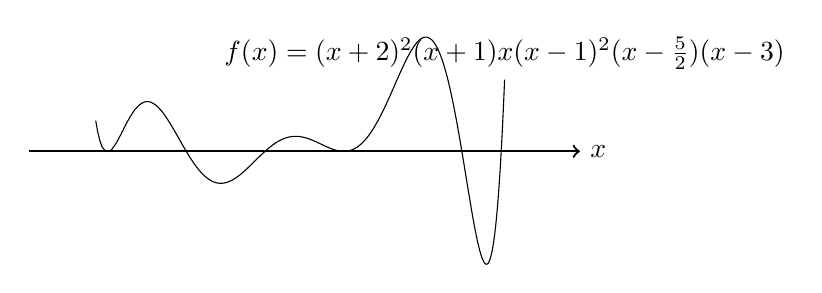
\begin{tikzpicture}
        % \draw[very thin,color=gray] (-0.1,-1.1) grid (3.9,8.1);
        \draw[->,thick] (-3,0) -- (4,0) node[right] {$x$}; 
        
        % \draw[domain=-6:6.5,samples=200] plot (\x,{sin((3*\x) r)});% node[right] {$f(x) = \sin x$};
        \draw[domain=-2.15:3.05,samples=500] plot (\x,{0.03*(\x+2)^2*(\x+1)*\x*(\x-1)^2*(\x-2.5)*(\x-3)}) node[above] {$f(x) = (x+2)^2(x+1)x(x-1)^2(x-\frac{5}{2})(x-3)$};
    \end{tikzpicture}
\end{center}

\end{enumerate}

考点三、含绝对值不等式的解法
\begin{enumerate}
    \item 最简单的绝对值不等式的同解变形;
    $$
    |ax+b|<c \Leftrightarrow -c<ax+b<c 
    $$
    $$
    |ax+b|>c \Leftrightarrow ax+b<-c \text{\  或 \ }  ax+b>c
    $$
    \item 不等式$ |x|<a\ (a>0)$的解集就是求在数轴上到原点的距离小于$a$的点对应的实数$x$的集合.

\end{enumerate}

\section{第8课\quad 基本不等式及其应用}
考点一、平均值不等式


\end{document}